\section{Anhang}
\begin{ctabular}{l|cccccc}
    \textbf{Hex} & A & B & C & D & E & F \\
    \textbf{Dec} & 10 & 11 & 12 & 13 & 14 & 15 \\
    \textbf{Bin} & 1010 & 1011 & 1100 & 1101 & 1110 & 1111
\end{ctabular}

\textbf{Parallel:}
Baudrate: $f_{\rm Baud} = \frac{1}{100\mu s} = 10'000 \text{ Baud}$ \\
Bitrate: $f_{\rm Bit} = \frac{8}{100\mu s} = 80'000 \text{ Bit/s}$

\textbf{Seriell:}
Baudrate: $f_{\rm Baud} = \frac{1}{100\mu s} = 10'000 \text{ Baud}$ \\
Bitrate: $f_{\rm Bit} = \frac{1}{100\mu s} = 10'000 \text{ Bit/s}$

\vspace{0.5em}
\noindent\textbf{Frequenzabweichung:} \\
Damit die Funktion gewährleistet werden kann, darf bei der Übertragung eines Frames die maximale Abweichung höchstens 1 Bitbreite betragen.
$$ f_{c,i} = \left(1 \pm \frac{\Delta t_{\rm max}}{t_{\rm max}}\right) * f_{2,i} = \left(1 \pm \frac{1 \text{ Bit}}{2 \cdot \text{Framelänge}}\right) * f_{c,i} $$

\vspace{0.5em}
\subsection{Oversampling: Voraussetzungen}
Die Mittelung von $M$ Samples bringt nur dann mehr Auflösung, wenn der ADC-Code zwischen Nachbarwerten \textbf{springt}:
\begin{itemize}
    \item \textbf{Mittelwertfreies Rauschen} (oder künstliches Dither-Signal) ist dem Eingang überlagert, Amplitude $\gtrsim 1$\,LSB.
    \item Rauschen \textbf{unkorreliert} von Sample zu Sample.
    \item Messsignal bleibt während der $M$ Samples \textbf{konstant}.
\end{itemize}
\vspace{-0.6em}
\begin{center}
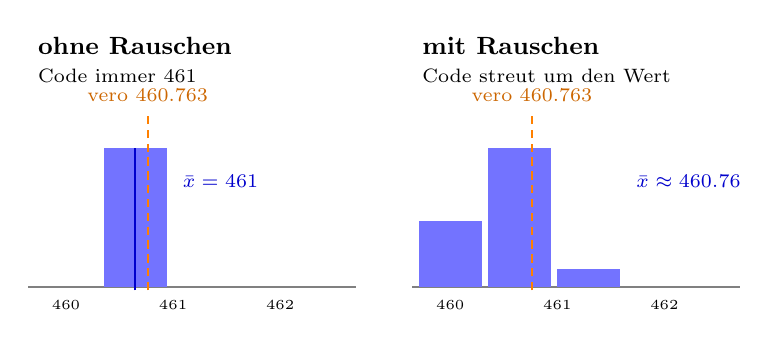
\begin{tikzpicture}[x=0.4cm,y=0.42cm,font=\scriptsize]
    % ohne Rauschen
  \begin{scope}
    \draw[gray] (0,0)--(10.4,0);
    \foreach \c [count=\i from 0] in {460,461,462}{\node at ({1.2+3.4*\i},-0.55) {\tiny\c};}
    \fill[blue!55] (2.4,0) rectangle (4.4,4.2);
    \draw[orange,thick,densely dashed] ({1.2+3.4*0.763},-0.1)--({1.2+3.4*0.763},5.3);
    \node[orange!80!black,anchor=south] at ({1.2+3.4*0.763},5.3) {vero 460.763};
    \draw[blue!80!black,thick] (3.4,-0.1)--(3.4,4.2);
    \node[blue!80!black,anchor=west] at (4.6,3.2) {$\bar x=461$};
    \node[anchor=west,font=\small\bfseries] at (0,7.3) {ohne Rauschen};
    \node[anchor=west] at (0,6.4) {Code immer 461};
  \end{scope}
  % mit Rauschen
  \begin{scope}[shift={(12.2,0)}]
    \draw[gray] (0,0)--(10.4,0);
    \foreach \c [count=\i from 0] in {460,461,462}{\node at ({1.2+3.4*\i},-0.55) {\tiny\c};}
    \fill[blue!55] (0.2,0) rectangle (2.2,2.0);
    \fill[blue!55] (2.4,0) rectangle (4.4,4.2);
    \fill[blue!55] (4.6,0) rectangle (6.6,0.55);
    \draw[orange,thick,densely dashed] ({1.2+3.4*0.763},-0.1)--({1.2+3.4*0.763},5.3);
    \node[orange!80!black,anchor=south] at ({1.2+3.4*0.763},5.3) {vero 460.763};
    \node[blue!80!black,anchor=west] at (6.8,3.2) {$\bar x\approx460.76$};
    \node[anchor=west,font=\small\bfseries] at (0,7.3) {mit Rauschen};
    \node[anchor=west] at (0,6.4) {Code streut um den Wert};
  \end{scope}
\end{tikzpicture}
\end{center}
\vspace{-0.6em}
\textbf{Ohne Rauschen} liefert der ADC immer denselben Code: die Mittelung gibt nur diesen zurück, die Information \glqq wie hoch genau\grqq{} ist verloren. \textbf{Mit Rauschen} streuen die Codes je nach Lage des wahren Wertes im Gradienten, der Mittelwert nähert sich ihm mit wachsendem

% --------------- Added in quickreference (screenshot) ---------------
% ---------------------- if necessary uncomment ----------------------
% \subsection{Bit-Shifting HEX}

% \begin{center}
% \renewcommand{\arraystretch}{1.3}
% \begin{tabular}{|c|l|}
% \hline
% \textbf{Operazione} & \textbf{Trucco a mente (hex)} \\
% \hline
% $x \ll 4$ & Aggiungi uno \texttt{0} in coda \\
% \hline
% $x \ll 1$ & Raddoppia cifra per cifra (da destra), \\
%  & riporto $+1$ se cifra $\geq 8$ \\
% \hline
% $x \ll 5$ & $(x\ll4)\ll1$: zero in coda, poi raddoppia \\
% \hline
% \hline
% $x \gg 4$ & Togli l'ultima cifra hex \\
% \hline
% $x \gg 1$ & Dimezza cifra per cifra (da sinistra), \\
%  & se riporto in entrata: $+8$ al risultato; \\
%  & riporto in uscita $=1$ se cifra dispari \\
% \hline
% $x \gg 5$ & $(x\gg4)\gg1$: togli ultima cifra, poi dimezza \\
% \hline
% \end{tabular}
% \end{center}

% \textbf{Tabella dimezzamento (per $\gg 1$):}
% \begin{center}
% \begin{tabular}{|c|c|c|}
% \hline
% cifra & metà & riporto generato \\
% \hline
% 0,2,4,6,8,A,C,E (pari) & $d/2$ & no \\
% 1,3,5,7,9,B,D,F (dispari) & $\lfloor d/2 \rfloor$ & sì $\to +1$ \\
% \hline
% \end{tabular}
% \end{center}